\documentclass[10pt,a4paper]{article}





%\usepackage{a4wide}
\usepackage[left=2.50cm, right=2.50cm, top=2.50cm, bottom=2.50cm]{geometry}
\usepackage{bm}
\usepackage{natbib}
\usepackage{amsmath}
\usepackage{amssymb}
\usepackage{listings}
\usepackage{graphicx}
\usepackage{epigraph}



\usepackage[T1]{fontenc}





\input NewCommands

\newcommand{\braket}[2]{\left \langle #1 \middle| #2 \right \rangle}

\DeclareMathOperator{\sgn}{sgn}


\begin{document}
\title{Subglacial hydrology}
\maketitle

\section{Basic equation of subglacial hydrology}
The background is explained in UaCompendium. For a groundwater flow
within a layer, the vertically integrated conservation equation of
water reads
\begin{equation}
  \frac{S_w}{\rho g} \p_t \phi + \nabla \cdot \bm{q}_w  = a_w \; 
\label{eq:hydphi}
\end{equation}
where $S_w$ is the \emph{storativity}, or the \emph{storage
coefficient}. Typically when considering subglacial hydrology, the
conceptual picture is that of an effective basal water layer of thickness $h_w$ for which mass conservation leads to
\begin{equation}
  \p_t h_w + \nabla \cdot \bm{q}_w  = a_w \; 
\label{eq:hwcon}
\end{equation}



For simplicity, here using a linear Darcy law where
\[
\bm{q}_w = -k h_w \nabla \phi
\]
and 
\[
\bm{v}_w= - k \nabla \phi
\]
and the hydraulic potential, $\phi$, is
\begin{align}
  \phi & = g \rho_w B + g \rho_w h_w + p_w  \label{eq:phi1} \\
  & = g \rho_w B + g \rho_w h_w + g \rho_i h - N \nonumber \\
    & = g \rho_w B + g \rho_w h_w + g \rho_i (s-b) - N \nonumber \\
  & = g \rho_w B + g \rho_w h_w + g \rho_i (s-(B+h_w))  - N \nonumber \\
  & = g (\rho_w-\rho_i) B + g \rho_i s +  g (\rho_w-\rho_i)  h_w  - N \label{eq:phi2}
\end{align}
or
\[
  \phi = \underbrace{g (\rho_w-\rho_i) B + g \rho_i s}_{=:\Phi} +  \underbrace{g (\rho_w-\rho_i)  h_w}_{=:\Upsilon}  - N 
  \]
that is
\[
\phi=\Phi + \Upsilon - N 
\]
where
\[
p_w=\rho_i g (s-b) -N
\]
which defines the effective pressure, $N$, as the deviation of the
water pressure, $p_w$, at the top of the water layer, from the ice
overburden presure, and where
\[
b=B+h_w \; .
\]
We have
\[
\partial_t h_w  + \nabla \cdot (k h_w \nabla (N-\Upsilon)) = a_w + \nabla \cdot (k h_w \nabla \Phi )
\]
or
\begin{equation}
\partial_t h_w  + \nabla \cdot (k h_w \nabla N) - \nabla \cdot ( \kappa h_w \nabla h_w ) = a_w + \nabla \cdot (k h_w \nabla \Phi )
\label{eq:hwEv}
\end{equation}
where
\[
\kappa:= k g (\rho_w-\rho_i)
\]
Equation (\ref{eq:hwEv}) has two unknowns, the effective water
pressure, $N$, and the water film thickness $h_w$. To close the system
we therefore need an additional evolutionary equation for the water
film thickness $h_w$. Typically this evolutionary equation involves the
effective pressure, $N$, and possibly the basal sliding velocity and
some aspects of the basal topography, i.e.\
\begin{equation}
h_w=f(N,\bm{v}_b,b)
\label{eq:hwdyn}
\end{equation}
The dynamics of the subglacial water flow will primarily be
determined by the nature of this functional relationship.

\section{Simplifications for water routing purposes}

Various simplifications of Eq.~(\ref{eq:hwEv}) and (\ref{eq:hwdyn})
have been proposed.

\subsection{$N=\Upsilon=0$}
For example in \cite{LeBrocq2009} it is assumed
that the effective water pressure is zero, i.e. that
\[
N=0
\]
and that $\phi$ does not depend on the water-film thickness, i.e.\ that
\[
\Upsilon=0
\]
With these simplifications Eq.~(\ref{eq:hwEv}) becomes
\begin{equation}
\partial_t h_w  = a_w + \nabla \cdot (k h_w \nabla \Phi )
\label{eq:hwEvALB}
\end{equation}
\cite{LeBrocq2009} used a different form of the Darcy flow equation, resulting in
\begin{equation}
\partial_t h_w  = a_w + \frac{1}{12 \mu} \nabla \cdot (h_w^2 \nabla \Phi) 
\label{eq:hwEvALB}
\end{equation}
that is
\begin{equation}
\partial_t h_w  = a_w + \frac{1}{12 \mu} \nabla \cdot (h_w^2 \nabla (g (\rho_w-\rho_i)B + \rho_i s))
\label{eq:hwEvALB2}
\end{equation}
Since the potential $\Phi$ does not depend on the water-film
thickness, $h_w$, the direction of the water velocity
\[
\bm{v}_w = \frac{h_w}{12 \mu} \nabla \Phi
\]
can not change over time in this model. It is therefore unclear how
this model can describe the filling of local depressions in the water
potential $\Phi$.
\]
\cite{LeBrocq2009} used a filling algorithm to get rid of `sinks' in
hydraulic potential, but it is unclear how this resulting in
modification of the algorithm used. Possibly, instead of using the expression 
\[
  \Phi= g (\rho_w -\rho_i) B + g \rho_i s \\
\]
the field $\Phi$ itself was modified. \cite{LeBrocq2009} furthermore
state that the `this algorithm suffers from dependency on the grid
size and orientation''.

\subsection{$N=0$ and $\Upsilon\neq0$}
It the overall geometry of the ice sheet. e.g.\ the bedrock $B(x,y)$
the upper surface $s(x,y)$, does not change over time, then the
direction of the water flow velocity, $\mb{v}_w$ can only change if
either, or both, the effective water pressure $N$ or the water film
thickness, $h_w$, evolve with time. For water-routing purposes it is
possible that sufficiently realistic predictions can be obtained by
allowing the water film thickness to evolve while setting the
effective pressure to zero, i.e.\
\begin{align*}
  N&=0 \\
  \Upsilon &\neq 0
\end{align*}
Equation (\ref{eq:hwEv}) then reads
\begin{equation}
  \partial_t h_w   - \nabla \cdot ( \kappa h_w \nabla h_w ) - \nabla \cdot (k h_w \nabla \Phi ) = a_w 
\label{eq:hwU}
\end{equation}
or
\begin{equation}
  \partial_t h_w   - \nabla \cdot\left (  k h_w \nabla (\Upsilon + \Phi ) \right )  = a_w 
\label{eq:hwD}
\end{equation}
where as before
\begin{align*}
  \Phi&:= g (\rho_w -\rho_i) B + g \rho_i s \\
  \Upsilon&:= g (\rho_w-\rho_i)  h_w  \\
  \kappa&:= k g (\rho_w-\rho_i)
\end{align*}
and we are using the approximation, $N=0$, in which cawse 
\[
\phi = \Upsilon +\Phi
\]
The water flux is
\begin{align*}
  \bm{q}_w & = -k h_w \nabla \phi\\
           & = -k h_w \nabla (\Upsilon + \Phi)\\
\end{align*}

Equation (\ref{eq:hwD}) is a non-linear diffusion equation and the finite-element system is
\[
\braket{(h_w^1 - h_w^0)}{\psi}    = \Delta t \,\braket{a_w}{\psi} - \Delta t \, \braket{k h_w \nabla (\Upsilon + \Phi )}{\psi} + \text{BT}
\]
The terms on the right-hand side are evaluated at $t=t_0$ and $t=t_1$
using the $\Theta$ method. Setting the boundary term, $\text{BT}=0$,
correspondes to a no-flux Neumann type boundary condition. In addition
$h_w$ can also be prescribed directly along the boundary, or at any
location within the computatinal domain (Dirichlet boundary
condition). Dirichlet conditions are implemented using Lagrange
multipliers. The positive thickness constraint
\[
h_w \ge 0
\]
is enforced using the active set method, and the resulting non-linear
KKT system is solved using the Newton-Raphson method.

\subsection{Remark on flotation}

Because of the assumption $N=0$, Eq.~(\ref{eq:hwU}) the ice is at
floatation. For $a_w=0$, the steady-state relationship between $s$ and
$b$ is then as expected for floating ice. To see this set $a_w=0$, $\p_t
h_w=0$, and insert
\begin{align*}
h_w&=b-B \\
\Phi&:= g (\rho_w -\rho_i) B + g \rho_i s \\
\end{align*}
in Eq.~(\ref{eq:hwU}), giving
\[
 \nabla b =  -\frac{\rho_i}{\rho_w-\rho_i} \nabla s 
\]
if $b=h_w+B$ is allowed to evolve.


Generally, in steady state, for $\Phi$ given and $a_w=0$, we have
\begin{equation}
\nabla h_w  = -\frac{1}{g (\rho_w-\rho_i)} \nabla \Phi 
\label{eq:hwUss2}
\end{equation}
or
\begin{align*}
  \nabla \Upsilon &= g (\rho_w-\rho_i) \nabla h_w  \\
                  &= -\nabla \Phi
\end{align*}
and therefore
\[
q_w= -k h_w \nabla (\Upsilon + \Phi) =0
\]
as expected for $a_w=0$.


\begin{figure}
\centerline{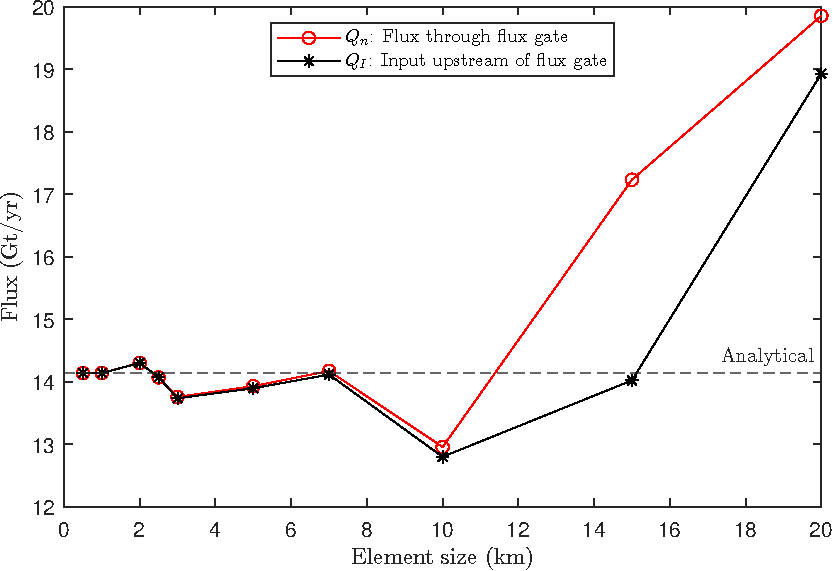
\includegraphics[width=12cm]{IslandConvergenceTest.pdf}}
\caption[Convergence test]{Mass conservation convergence test. The
  geometry is that of a dome-shaped island surrounded by ocean. A
  constant water flux, $a_w=10\,\mathrm{m\,yr^{-1}}$, is added within a semi-circle of a given
  radius, $r_w=30\,\mathrm{km}$, so that the total water added is
  $Q_{\mathrm{analytical}}=\pi a_w
  r_w^2/2=14.1372\,\mathrm{Gt\,yr^{-1}}$. A flux gate is defined as a
  circle downstream of $r_w$ and the total integrated flux through the
  gate, $Q_n$, is evaluated numerically and compared with the
  analytical value, $Q_{\mathrm{analytical}}$. A comparision is also
  made with the numerically integrated water input, $Q_I$. For the
  smallest element size of 0.5 km, the numerical flux through the flux
  gate is $Q_n=14.1386\,\mathrm{Gr\,yr^{-1}}$, or an error of 0.011\%.
\label{fig:IslandCon}}
\end{figure}



\section{MATLAB files}

Here a short summary is
provided of the equations solved by the m-files. The main assumption
here is that the effective pressure is zero, i.e.\ $N=0$, and that the
water flow is confined to a layer of variable thickness, $h_w$.

\bigskip
\textbf{GroundWaterEquation.m}

For a groundwater flow within a layer, the vertically
integrated conservation equation of water reads
\begin{equation}
  \frac{S_w}{\rho g} \p_t \phi + \nabla \cdot \bm{q}_w  = a_w \; 
\label{eq:hydphi}
\end{equation}
where $S_w$ is the \emph{storativity}, or the \emph{storage coefficient}. Using a linear Darcy law where
\[
\bm{q}_w = -k h_w \nabla \phi
\]
and 
\[
\bm{v}_w= - k \nabla \phi
\]
and (see Eq.~(\ref{eq:phi2} below) 
\[
  \phi = \underbrace{g (\rho_w-\rho_i) B + g \rho_i s}_{=:\Phi} +  \underbrace{g (\rho_w-\rho_i)  h_w}_{=:\Upsilon}  - N 
  \]
  that is
\[
\phi=\Upsilon - N +\Theta
\]
We have
\[
\frac{S_w}{\rho g}  \partial_t (N-\Upsilon)  + \nabla \cdot (k h_w \nabla (N-\Upsilon)) = a_w + \nabla \cdot (k h_w \nabla \Phi )
\]
This equation has two unknowns, the effective water pressure (N), and
the water film thickness $h_w$. To close the system we therefore need
an additional evolutionary equation for the water film thickness
$h_w$. Typically this evolutionary equation involves the effective
pressure, $N$, and possibly the basal sliding velocity and some aspects of the basal topography, i.e.\
\[
h_w=f(N,\bm{v}_b,b)
\]



Solves
\[
\frac{S_w}{\rho g}  \partial_t N +  \bm{v}_w \cdot \nabla N  + \nabla \cdot (\kappa h_w \nabla N) = a_w + \nabla \cdot (k h_w \nabla \Phi )
\]
where
\[
\Phi = (\rho_w-\rho) g \nabla b - \rho g \nabla s
\]




\medskip
\textbf{WaterFilmThicknessEquation.m }

Solves for the water-film thickness, $h_w$ of confined aquifer with a
variable water film thickness using
\[\partial_t h_w +   \nabla \cdot ( \bm{q}_w ) = a_w \]
the water flux is


\begin{equation}
\bm{q}_w=  - k h_w \nabla \phi
\label{eq:Df}
\end{equation}
and
\begin{align}
  \phi & = g \rho_w B + g \rho_w h_w + p_w  \label{eq:phi1} \\
  & = g \rho_w B + g \rho_w h_w + g \rho_i h - N \nonumber \\
    & = g \rho_w B + g \rho_w h_w + g \rho_i (s-b) - N \nonumber \\
  & = g \rho_w B + g \rho_w h_w + g \rho_i (s-(B+h_w))  - N \nonumber \\
  & = g (\rho_w-\rho_i) B + g \rho_i s +  g (\rho_w-\rho_i)  h_w  - N \label{eq:phi2}
\end{align}
or
\begin{equation}
\phi= \Phi +  \Upsilon - N\; .
 \label{eq:hwEq}
\end{equation}
with
\begin{equation}
  \Phi := (\rho_w - \rho_i) g B  +  \rho_i g s \; ,
 \label{eq:Phidef2}
\end{equation}
and
\begin{equation}
  \Upsilon := g (\rho_w-\rho_i)  h_w  \; ,
 \label{eq:Phidef3}
\end{equation}
Setting $N=0$ and adding an optional linear diffusion term, leads to
\[
\bm{q}_w =   h_w \bm{v}_w   -   \kappa h_w \nabla h_w   -   \eta  \nabla h_w \]
that is
\[
\partial_t h_w +  \nabla \cdot (  h_w \bm{v}_w )  - \nabla \cdot (\kappa h_w \nabla h_w) -\nabla \cdot (\eta \nabla h_w )= a_w
\]
Here the water velocity, $\bm{v}_w$, is prescribed, and $\kappa=k g
(\rho_w-\rho_i)$. In the m-file some flags have been introduced for switching individual terms on and off ($\alpha$ and $\beta$ flags).
 
\medskip
\textbf{WaterFilmVelocities.m}

Returns the water velocities $\bm{v}_w$ of the confined aquifer. This can, for example, be done as
\[ \bm{v}_w= - k \nabla \Phi \]
or by prescribing the $\bm{v}$ directly.

\medskip
\textbf{PhiPotential.m}
Calculates the potential $\Phi$ which is

\[
\Phi = g \left ( (\rho_w-\rho_i) B + \rho_i  s \right )   \]

\medskip




\clearpage
\bibliographystyle{apalike}


\bibliography{../../../Handouts/UaCompendium.bib}

%\bibliography{glacier}
%\bibliography{library,glacier}
%\bibliography{library}



\end{document}
